\chapter{\label{ch:4-qd-method}A scalable variational inference approach for increased mixed-model association power}

\minitoc

\section{Chapter overview}
In this chapter, we introduce a novel method called Quickdraws, which we developed to perform scalable and statistically powerful genome-wide association studies. Quickdraws leverages advancements in machine learning and the processing power of modern computing architectures, such as graphical processing units (GPUs), to conduct genome-wide association studies on a large scale. We begin by presenting the theoretical framework for Quickdraws in section \ref{sec:ch4-theory}, which incorporates modern variational inference techniques, including stochastic variational inference. After establishing the theoretical foundation, we will delve into the algorithm's details in section \ref{sec:ch4-method}, covering several steps such as heritability estimation, Bayesian regression, and the estimation and calibration of test statistics. Finally we summarize the key steps in the algorithm in section \ref{sec:ch4-summary}.

\begin{figure}[h!]
    \centering
    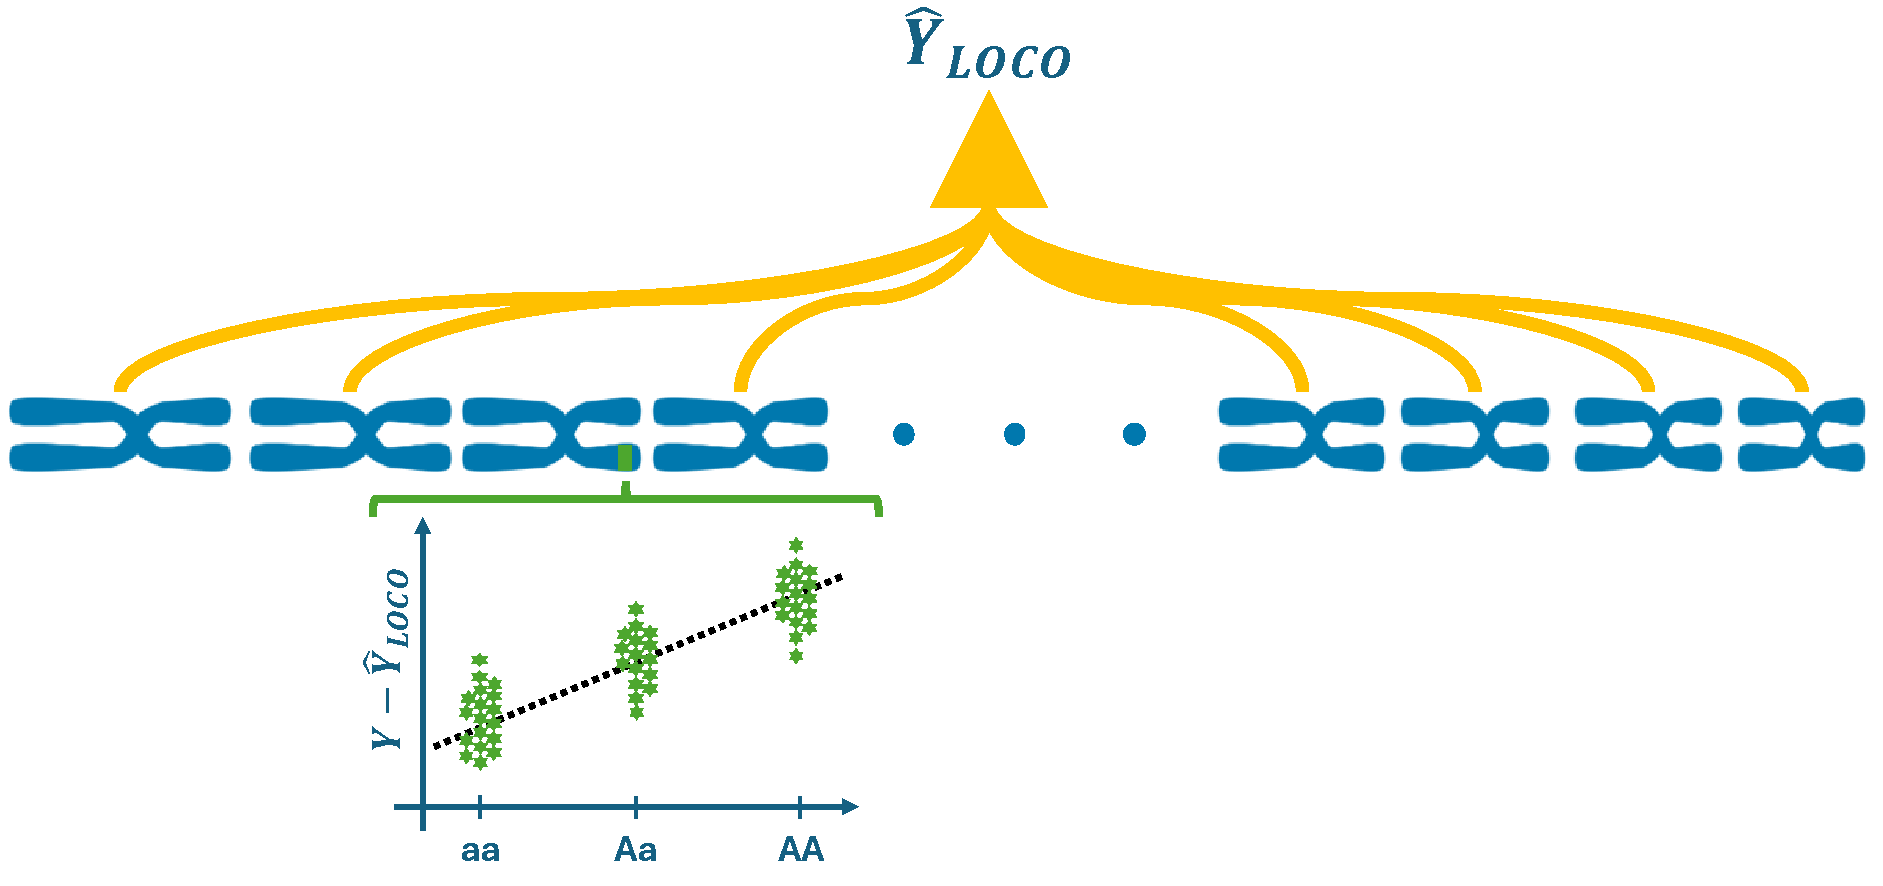
\includegraphics[width=\textwidth]{figures/thesis_qd_simplified_overview.pdf}
    \caption{\textbf{A simplified overview of Quickdraws.} Quickdraws is a scalable mixed model designed for genome-wide association studies (GWAS). It improves the power of association testing through a two-step process. First, it estimates the genomic prediction for a trait by excluding the testing chromosome, employing a leave-one-chromosome-out method. The prediction models sparsity of effects and is optimized using advanced variational inference techniques ensuring scalability for large sample sizes. Second, the model leverages this genomic prediction to improve the signal-to-noise ratio for finding association between a trait and a variant.}
    \label{fig:qd-simplified-overview}
\end{figure}

\section{Theoretical framework for our method}
\label{sec:ch4-theory}
\subsection{Bayesian inference}
Bayesian inference is a popular statistical inference approach that takes into account prior beliefs about the model along with evidence obtained from the data.
%
We introduce some basic terminology related to Bayesian inference, which we utilize in the following sections to describe our inference approach.
%
We refer the reader to \cite{blei2017variational,bishop2006pattern} for a more in-depth review on Bayesian inference and variational Bayes approaches.
%
We use the following notation and terminology:
%
\begin{itemize}
    \item $X = (x_1, x_2, ..., x_n)$ is a set of $n$ observed data-points 
    \item $\theta$ parameterizes the probability distribution of the data-points, $x \sim P(x \mid \theta)$.
    \item The \textbf{prior} distribution, $P(\theta)$, is the distribution of the parameters before any data is observed.
    \item The \textbf{data likelihood} or likelihood, $P(X \mid \theta)$, is the distribution of the data conditioned on model parameters.
    \item The \textbf{evidence} or marginal likelihood is the distribution of the observed data marginalized over parameters,
    \begin{equation}
        P(X) = \int P(X \mid \theta) P(\theta) d \theta \nonumber.
    \end{equation} 
    
    \item The \textbf{posterior}, $P(\theta \mid X)$, is the distribution of the parameters after taking into account the observed data,
    \begin{equation}
        P(\theta \mid X) = \frac{P(X \mid \theta) P(\theta)}{P(X)} = \frac{P(X \mid \theta) P(\theta)}{\int P(X \mid \theta) P(\theta) d \theta} \nonumber.
    \end{equation}
    
\end{itemize}
%

%
In the context of Bayesian inference, we are most interested in deriving the posterior distribution given prior beliefs on the parameters.
%
Unless the likelihood and prior are conjugate, however, we generally cannot derive a closed-form solution for the posterior.
%
Thus, in more general and usually more complex scenarios, Bayesian Inference heavily relies on sampling approaches, such as MCMC, or approximate methods, such as variational Bayes, to infer the posterior.
\subsection{Variational inference}
Variational inference is a popular approximate inference technique often used to infer posterior estimates for models that do not allow for a closed-form solution for their posterior.
%
In variational inference, posterior inference is formulated as an optimization problem.
%
As the exact posterior probability is often intractable, we assume an approximate posterior family that is easy to evaluate.
%
We then optimize the parameters of this posterior family so that the Kullback–Leibler (KL) divergence between the approximate and true posteriors is sufficiently small:
\begin{equation}
    KL\left(q_{\omega} (\theta) \| P(\theta \mid X) \right) = \int q_{\omega} (\theta) \log \left( \frac{q_{\omega} (\theta)}{P(\theta \mid X)} \right) d \theta \label{kl},
\end{equation}
where $P(\theta \mid X)$ is the true posterior and $q_{\omega} (\theta)$ is the approximate posterior, parameterized by $\omega$ (also known as variational parameters).
%
Variational inference aims to minimize the KL divergence in Equation \ref{kl}, to obtain optimal variational parameters $\omega^{*}$: 
\begin{equation}
    \omega^{*} = \underset{\omega}{\mathrm{argmin}}KL(q_{\omega}(\theta)||P(\theta|\textbf{X})).
    \label{opti}
\end{equation}

\subsection{Evidence lower bound and mean-field variational inference}
\label{sec:ch4-theory-mfvi}
Note that Equation \ref{opti} poses an optimization problem that requires the calculation of KL divergence between approximate posterior and the true posterior.
%
However, this objective cannot be computed because it requires information about the posterior, which is not available in closed form.
%
We thus use the Bayes rule to simplify the above equation,
%

\begin{align}
    KL(q_{\omega}(\theta)||P(\theta|\textbf{X})) &= \mathbb{E}[log(q_{\omega}(\theta))] -\mathbb{E}[log(P(\theta|\textbf{X})] \nonumber \\
&= \mathbb{E}[log(q_{\omega}(\theta))] -\mathbb{E}[log(P(\theta,\textbf{X})] + log(P(\textbf{X})) \nonumber \\
& = KL(q_{\omega}(\theta)||P(\theta)) -  \mathbb{E}[log(P( \textbf{X}|\theta)] + log(P(\textbf{X})) \geq 0
\end{align} 
\begin{equation}
    \implies log(P(\textbf{X})) \geq \mathbb{E}[log(P( \textbf{X}|\theta)] - KL(q_{\omega}(\theta)||P(\theta)) \label{elbo_bound}.
\end{equation}

%
In the above, the term on the left is the logarithm of the evidence, so the term on the right is called the evidence lower bound, or ELBO.
%
Variational inference algorithms try to minimize the KL divergence between the true posterior and approximate posterior by maximizing the ELBO in Equation \ref{elbo_bound}.
%
The ELBO can also be seen as the difference between the expected log-likelihood of the data and the KL divergence between the approximate posterior and prior,
\begin{equation}
    \mathcal{L}_{VI}(\omega) = \mathbb{E}[log(P( \textbf{X}|\theta)] - KL(q_{\omega}(\theta)||P(\theta)).
\end{equation}

%
In the context of Bayesian regression, our sampling distribution is $P(y \mid X)$ instead of $P(X)$, where $y$ is the outcome variable and $X$ is the input variable.
%
In that case, the ELBO is written as
\begin{equation}
    \mathcal{L}_{VI}(\omega) = \underbrace{\mathbb{E}[\log(P( \textbf{y}|\theta, \textbf{X}))]}_{\text{Expected LL}} - \underbrace{KL(q_{\omega}(\theta)||P(\theta))}_{\text{KL-divergence}}
    \label{elbo_blr}
\end{equation}

\subsubsection{Mean-field variational inference}

The fully-factorized or mean-field posterior is a commonly used approximate posterior in variational inference.
%
In this approach, the posterior can be represented as a product of factors with only one parameter per factor.
%
This enables the use of coordinate-ascent variational inference algorithms and makes operations such as sampling and computation of the ELBO, used in other variational inference strategies, more efficient.
%

%
Using this approach, the model we adopt when estimating genetic effects in quantitative traits, i.e., a Bayesian linear regression with spike-and-slab prior and a fully-factorized spike-and-slab approximate posterior, takes the form
\begin{align}
    &\text{\textbf{Likelihood:} } &P(y \mid X, \beta) \sim \mathcal{N}(\beta^T X, \sigma_e^2) \nonumber \\
    &\text{\textbf{Prior:} } &P(\beta) = \prod_j P(\beta_j), \hspace{1mm} P(\beta_j) \sim (1-p_0)\mathcal{N} (0, \sigma ^ 2) + p_0 \delta(0) \nonumber \\
    &\text{\textbf{Approximate Posterior:} } &q(\beta) = \prod_j q(\beta_j), \hspace{1mm} q(\beta_j) \sim (1-\psi_j)\mathcal{N}(\mu_j, \sigma^2_j) + \psi_j \delta(0)
    \label{spike-and-slab-model}
\end{align}

In the above, $y$ and $X$ are the output and input variables, respectively, $\beta$ are the unknown effects of the linear regression, which have a spike-and-slab prior $P(\beta)$, $\sigma_e^2$ and $\sigma^2$ are the variance component corresponding to noise and per predictor effect, $p_0$ is the sparsity and $j$ indexes all the predictors in the regression.
%
The approximate posterior in this model assumes a fully-factorized spike-and-slab structure with variational parameters $\mu$, $\psi$, and $\sigma$.
%
As shown in \cite{spence2020flexible}, a spike-and-slab prior is conjugate to the normal likelihood, making a fully-factorized spike-and-slab posterior a good choice for the approximate posterior family. 

\subsection{Coordinate ascent variational inference}
Coordinate ascent variational inference (CAVI), introduced in \cite{bishop2006pattern}, is one of the most popular mean-field variational inference algorithms.
%
CAVI iteratively optimizes each factor in the mean-field posterior while fixing the other factors, thereby improving the ELBO in each iteration and finding a local optimum.
%
CAVI updates each factor in the approximate posterior as follows:
\begin{equation}
    \log q(\beta^{*}{_j}) = E_{\beta_{(-j)}} [\log(P(y, \beta))] + C \label{cavi}
\end{equation}

%
The optimal update for a variational parameter is proportional to the exponential of the expected logarithm of the complete conditional, where the expectation is taken with respect to all the variational parameters except the one which is being updated.
%
It can be shown that the above updates increase the ELBO each iteration (see \cite{blei2017variational} for a concise proof).
%
We next derive the CAVI update equations for the Bayesian linear regression model described in Equation \ref{spike-and-slab-model}.
%

\newpage

%
\noindent \textbf{Derivation of CAVI updates for spike-and-slab Bayesian linear regression:}

\begin{align}
    \log q(\beta^{*}{_j}) &= E_{\beta_{(-j)}} [\log(P(y, \beta))] + C \nonumber \\
    &= E_{\beta_{(-j)}} \log P(y \mid \beta) + E_{\beta_{(-j)}} \log P(\beta_j) + C \nonumber \\
    &= \sum_{n=1}^N \left( E_{\beta_{(-j)}} \log P(y_n \mid \beta) \right) + E_{\beta_{(-j)}} \log P(\beta_j) + C \label{cavi-1}.
\end{align}

%
To show this, we will ignore the terms in the complete conditional that do not depend on $\beta_j$ and simplify the complete conditional for $N$ data points.
%
We will also remove terms which do not depend on $\beta_j$ and absorb them in the constant $C$; the constant is thus not necessarily the same from one step to the other, but we simplify the notation by always expressing it as $C$.
%

%
We start by simplifying the equation by substituting the normal log-likelihood and spike-and-slab prior,
\begin{equation}
    \log q(\beta^{*}{_j}) = \sum_{n=1}^N E_{\beta_{(-j)}} \Big(- \frac{(y_n - \beta^T x_n)^2}{2 \sigma_e^2}  - log(\sigma_{e}) \Big)+ E_{\beta_{(-j)}}  \log P(\beta_j) + C.
\end{equation}

%
Because the spike-and-slab distribution can be seen as mixture of non-overlapping Gaussians, \cite{spence2020flexible} shows that it forms an exponential family (see theorems 1 and 2 in \cite{spence2020flexible}).
%
The natural parameters for the spike-and-slab distribution $(1-p_0) \mathcal{N}(\mu, \sigma^2) + p_0 \delta(0)$ are $-\frac{1}{2\sigma^2}$, $\frac{\mu}{\sigma^2}$, and $\log p_0 - \log (1-p_0) + \frac{\mu^2}{2\sigma^2} + \frac{1}{2}\log \sigma^2$, with corresponding sufficient statistics $\mathbb{I}\left\{\beta_j \ne 0\right\} \beta_j^2$, $\mathbb{I}\left\{\beta_j \ne 0\right\} \beta_j$, and $\mathbb{I}\left\{\beta_j = 0\right\}$.
%
We can substitute the natural parameters for the prior to simplify further:

\begin{align}
    &\log q(\beta^{*}_j) = \nonumber \\
    &= \sum_{n=1}^N E_{\beta_{(-j)}} \left( - \frac{(y_n - \beta^T x_n)^2}{2 \sigma_e^2} \right) + E_{\beta_{(-j)}} \bigg( - \mathbb{I}\left\{\beta_j \ne 0\right\} \frac{\beta_j^2}{2\sigma^2} \nonumber \\
    &\quad - \mathbb{I}\left\{\beta_j = 0\right\} \left(\log p_0 - \log (1-p_0) + \log(\sigma) \right)\bigg) + C \nonumber \\
    &= - E_{\beta_{(-j)}} \left( \frac{\sum_{n=1}^N (y_n - \beta_j x_{n,j} - \sum_{i \ne j} \beta_i x_{n,i})^2}{2 \sigma_e^2} \right)  - \mathbb{I}\left\{\beta_j \ne 0\right\} \frac{\beta_j^2}{2\sigma^2} \nonumber \\
    &\quad - \mathbb{I}\left\{\beta_j = 0\right\} \left(\log \frac{p_0 \sigma}{1-p_0} \right) + C \nonumber \\
    &= - E_{\beta_{(-j)}} \left( \frac{\sum_{n=1}^N (\beta_j x_{n,j} - (y_n - \sum_{i \ne j} \beta_i x_{n,i}))^2}{2 \sigma_e^2} \right)  - \mathbb{I}\left\{\beta_j \ne 0\right\} \frac{\beta_j^2}{2\sigma^2} \nonumber \\
    &\quad - \mathbb{I}\left\{\beta_j = 0\right\} \left(\log \frac{p_0 \sigma}{1-p_0} \right) + C \nonumber \\
    &= - E_{\beta_{(-j)}} \left( \frac{\sum_{n=1}^N (\beta^2_j x^2_{n,j} - 2(y_n - \sum_{i \ne j} \beta_i x_{n,i})\beta_j x_{n,j})}{2 \sigma_e^2} + \frac{\beta_j^2}{2\sigma^2} \right) \mathbb{I}\left\{\beta_j \ne 0\right\} \nonumber \\
    &\quad - \left(\log \frac{p_0 \sigma}{1-p_0} \right)\mathbb{I}\left\{\beta_j = 0\right\} + C \nonumber \\
    &= - \left( \frac{\sum_{n=1}^N x^2_{n,j}}{2 \sigma_e^2} + \frac{1}{2\sigma^2} \right)\mathbb{I}\left\{\beta_j \ne 0\right\}\beta_j^2  - \left(\log \frac{p_0 \sigma}{1-p_0} \right)\mathbb{I}\left\{\beta_j = 0\right\} \nonumber \\
    &\quad + E_{\beta_{(-j)}} \left( \frac{\sum_{n=1}^N (y_n - \sum_{i \ne j} \beta_i x_{n,i}) x_{n,j}}{\sigma_e^2} \right)\mathbb{I}\left\{\beta_j \ne 0\right\}\beta_j  + C
\end{align}

%
Substituting the expected value of the approximate spike-and-slab posterior $(1-\psi_i)\mathcal{N}(\mu_i, \sigma_i) + \psi_i \delta(0)$ with $(1-\psi_i)\mu_i$,

\begin{align}
   \log q(\beta^{*}{_j}) &=  {\color{red}{- \left( \frac{\sum_{n=1}^N x^2_{n,j}}{2 \sigma_e^2} + \frac{1}{2\sigma^2} \right)}}\mathbb{I}\left\{\beta_j \ne 0\right\}\beta_j^2 \nonumber +\\ & \hspace{4mm} {\color{blue}{+ \left( \frac{\sum_{n=1}^N (y_n - \sum_{i \ne j} \mu_i (1- \psi_i) x_{n,i}) x_{n,j})}{ \sigma_e^2} \right)}}\mathbb{I}\left\{\beta_j \ne 0\right\}\beta_j \nonumber +\\ & \hspace{4mm} {\color{green}{- \left(\log \frac{p_0 \sigma}{1-p_0} \right)}}\mathbb{I}\left\{\beta_j = 0\right\} + C.
\end{align}

%
Now comparing the coefficients of the sufficient statistics $\mathbb{I}\left\{\beta_j \ne 0\right\} \beta_j^2$, $\mathbb{I}\left\{\beta_j \ne 0\right\} \beta_j$ and $\mathbb{I}\left\{\beta_j = 0\right\}$ to the natural parameters of the spike-and-slab $-\frac{1}{2\sigma_j^2}$, $\frac{\mu_j}{\sigma_j^2}$ and $\log \psi_j - \log (1-\psi_j) + \frac{\mu_j^2}{2\sigma_j^2} + \frac{1}{2}\log \sigma_j^2$, respectively \cite{spence2020flexible}, we get the following update rules:

\begin{align}
    \sigma_j^2 &= \frac{1}{\frac{\sum_{n=1}^N x^2_{n,j}}{ \sigma_e^2} + \frac{1}{\sigma^2}} \nonumber \\
    \mu_j &= \frac{\sum_{n=1}^N (y_n - \sum_{i \ne j} \mu_i (1- \psi_i) x_{n,i}) x_{n,j})}{\sum_{n=1}^N x^2_{n,j} + \frac{\sigma_e^2}{\sigma^2}} \nonumber \\
    \psi_j &= 1 - \frac{1}{1 + \frac{p_0}{1-p_0}\sqrt{1 + \sigma^2 / \sigma_e^2 \sum_{n=1}^N x^2_{n,j} }  \exp\left\{ - \frac{\Big( \sum_{n=1}^N \left( y_n - \sum_{i \ne j} \mu_i (1- \psi_i) x_{n,i}) x_{n,j} \right) \Big)^2}{2\sigma_e^4/ \sigma^2 + 2\sigma_e^2\sum_{n=1}^N x^2_{n,j}}\right\}}
\label{eq:cavi_2_update_psi}
\end{align}

\subsection{Stochastic variational inference}
\label{sec:ch4-theory-svi}
%
CAVI provides a principled way to perform variational inference but requires a full pass through the data for each iteration, which is computationally expensive for large datasets.
%
BOLT-LMM \cite{loh2015efficient} \cite{loh2018mixed} observed that CAVI scales approximately as $\mathcal{O}(MN^{1.5})$, because the number of CAVI steps increase by $\sqrt{N}$, where $M$ is the number of predictors and $N$ is the number of samples.
%
Stochastic variational inference \cite{hoffman2013stochastic} uses ideas from stochastic optimization \cite{robbins1951stochastic} to update the variational parameters through a noisy but unbiased estimate of ELBO's gradient.
%
Like other modern machine learning optimizers, stochastic variational inference is also amenable to working with batches of data, rather than with a full pass through the data, making it more efficient when applied to large datasets.
%
Overall, stochastic variational inference provides a more efficient and scalable approach for posterior inference and has been widely applied to many machine learning problems, ranging from topic modeling \cite{hoffman2013stochastic} to generative models such as variational autoencoders (VAE) \cite{kingma2013auto}.
%

%
We now derive the stochastic variational inference objective for the Bayesian linear regression model described in Equation \ref{spike-and-slab-model} and a similar Bayesian logistic regression model.
%
In later section \ref{sec:ch4-blr}, we highlight several practical considerations linked to implementing the algorithm.
%

\newpage

\noindent \textbf{Derivation of Stochastic VI objective for spike-and-slab Bayesian linear regression:}
%

%
Stochastic VI tries to find the optimal variational parameters by performing gradient descent directly on the ELBO objective in Equation \ref{elbo_blr},
\begin{equation}
    L_{VI}(\psi, \mu, \sigma) = E[log(P( y \mid \beta,X)] - KL(q_{\psi, \mu, \sigma}(\beta) \mid P(\beta))
\end{equation}

%
Assuming the same model as in Equation \ref{spike-and-slab-model} with a fully factorized spike and slab prior, the ELBO can be simplified as follows:
\begin{align}
 L^{Q}_{VI}(\psi, \mu, \sigma) &= \sum\limits^{N}_{n=1} E[log(p(y_{n} \mid \beta))] - KL(q_{\psi, \mu, \sigma}(\beta) \mid P(\beta)) \nonumber \\
 &= \sum\limits^{N}_{n=1} E[log(p(y_{n} \mid \beta))] - \sum\limits^{M}_{j=1} KL(q_{\psi_j, \mu_j, \sigma_j}(\beta_j) \mid P(\beta_j)) \nonumber \\
 &= - \sum\limits^{N}_{n=1} \int \frac{(y_n - \beta^T x_n)^2}{2 \sigma_e^2} q_{\psi, \mu, \sigma}(\beta) d\beta - \sum\limits^{M}_{j=1} KL(q_{\psi_j, \mu_j, \sigma_j}(\beta_j) \mid P(\beta_j)) \label{spike-and-slab-1}
\end{align}
where $N$ is the number of samples, $M$ is the number of predictors, and $\beta$ are the effect estimates.
%
We derive the KL divergence between two spike-and-slab distributions as a special case of the KL divergence between non-overlapping mixture distributions (see Appendix \ref{app:1-KL_divergence} for details).
%
We do not have a closed form for the log-likelihood term.
%
The usual approach in stochastic variational inference is to replace the integral with an approximate monte-carlo estimate.
%
This results in a noisy yet unbiased estimate of the ELBO, which can be shown to converge to a local minimum under the Robbins-Munro condition \cite{robbins1951stochastic} on step-size:
\begin{align}
    L^{Q}_{VI}&(\psi, \mu, \sigma) \approx - \sum\limits^{N}_{n=1} \sum\limits^{S}_{s=1} \frac{(y_n - \beta(s) x_n)^2}{2 \sigma_e^2} + \nonumber \\
    &- \sum\limits^{M}_{j=1} \left(  \frac{\psi_j}{2}\left(-1 + \frac{\mu_j^2 + \sigma_j^2}{\sigma^2} - \log \frac{\sigma_j^2}{\sigma^2} \right) + (1-\psi_j)\log\frac{1 - \psi_j}{1 - p_0} + \psi_j\log\frac{\psi_j}{p_0} \right )
\end{align}

%
We take $S$ monte-carlo samples from the approximate posterior $\beta(s)$ to calculate the approximate log-likelihood.
%
Similar to the use of stochastic optimization in machine learning, we can also have a batched version of the above ELBO, where we update the variational parameters after each mini-batch of data.
%
We divide the input data into $B$ equally sized batches and maximize the batched-version of ELBO given below:
\begin{align}
    L^{Q}_{VI}&(\psi, \mu, \sigma) \approx - \sum\limits^{B}_{b=1} \Bigg( \sum\limits^{S}_{s=1} \frac{(y_b - \beta(s) X_b)^2}{2 \sigma_e^2} + \nonumber \\
    &+ \frac{1}{B}\sum\limits^{M}_{j=1} \left(  \frac{\psi_j}{2}\left(-1 + \frac{\mu_j^2 + \sigma_j^2}{\sigma^2} - \log \frac{\sigma_j^2}{\sigma^2} \right) + (1-\psi_j)\log\frac{1 - \psi_j}{1 - p_0} + \psi_j\log\frac{\psi_j}{p_0} \right) \Bigg)
    \label{elbo-loss}
\end{align}


%
\vspace{3mm}
\noindent \textbf{Derivation of Stochastic VI objective for spike-and-slab Bayesian logistic regression:}
\vspace{2mm}
%

%
The Bayesian logistic regression model is similar to the linear regression case, only differing in the likelihood term.
%
The model for Bayesian logistic regression with spike-and-slab prior can be written as
%

\begin{align}
    &\text{\textbf{Likelihood:} } &P(y \mid X, \beta) = \prod_{n=1}^{N} c_n^{y_n} \{1 - c_n\}^{1-y_n}, \hspace{1mm} c_n = \sigma(\beta^T X_n) \nonumber \\
    &\text{\textbf{Prior:} } &P(\beta) = \prod_j P(\beta_j), \hspace{1mm} P(\beta_j) \sim (1-p_0)\mathcal{N} (0, \sigma ^ 2) + p_0 \delta(0) \nonumber \\
    &\text{\textbf{Approximate Posterior:} } &q(\beta) = \prod_j q(\beta_j), \hspace{1mm} q(\beta_j) \sim (1-\psi_j)\mathcal{N}(\mu_j, \sigma^2_j) + \psi_j \delta(0)
    \label{spike-and-slab-model3-rep}
\end{align}

Similar to the linear model in equation \ref{spike-and-slab-model}, $X_n$ and $y_n$ represent the input vector and output values for the $n$-th datapoint.
%
We still assume a spike-and-slab approximate posterior, although it is not conjugate to the logistic regression model, because we empirically find it to still perform well in this case.
%
The ELBO for Bayesian logistic regression can be simplified as in the linear case:
\begin{small}
\begin{align}
 &L^{Bi}_{VI}(\psi, \mu, \sigma) = \sum\limits^{N}_{n=1} E[log(p(y_{n} \mid \beta))] - KL(q_{\psi, \mu, \sigma}(\beta) \mid P(\beta)) \nonumber \\
 &= - \sum\limits^{N}_{n=1} \int \{y_n \log c_n + (1-y_n)\log(1-c_n)\} q_{\psi, \mu, \sigma}(\beta) d\beta - \sum\limits^{M}_{j=1} KL(q_{\psi_j, \mu_j, \sigma_j}(\beta_j) \mid P(\beta_j))
\label{spike-and-slab-2}
\end{align}
\end{small}
where $c_n = \sigma(\beta^T X_n)$, i.e., the output after sigmoid activation.
%
We estimate the expected log-likelihood with a Monte Carlo estimate, whereas we write a closed-form solution for the KL divergence term similar to Equation \ref{elbo-loss}.
%
The batched version of the ELBO for Bayesian logistic regression can be written as
\begin{align}
    L^{Bi}_{VI}&(\psi, \mu, \sigma) \approx - \sum\limits^{B}_{b=1} \Bigg( \sum\limits^{S}_{s=1} y_b \log(\sigma(\beta^T X_b)) + (1-y_b)\log(1-\sigma(\beta^T X_b)) \nonumber +\\
    &+ \frac{1}{B}\sum\limits^{M}_{j=1} \left(  \frac{\psi_j}{2}\left(-1 + \frac{\mu_j^2 + \sigma_j^2}{\sigma^2} - \log \frac{\sigma_j^2}{\sigma^2} \right) + (1-\psi_j)\log\frac{1 - \psi_j}{1 - p_0} + \psi_j\log\frac{\psi_j}{p_0} \right) \Bigg)
\label{elbo-loss2}
\end{align}
where we take $S$ Monte Carlo samples to approximate the log-likelihood term.


\section{Method description}
\label{sec:ch4-method}
\subsection{Overview of the method}
Quickdraws is a mixed-model association algorithm that models phenotypes as a combination of fixed effects, random genetic effects, and random environmental effects (see section \ref{sec:ch1-lmm} for introduction to mixed models).
%
Like all modern GWAS algorithms \cite{loh2015efficient,loh2018mixed,zhou2018efficiently,jiang2019resource,jiang2021generalized,mbatchou2021computationally}, Quickdraws detects association using a two-step approach.
%
The first step, sometimes called model fitting, focuses on estimating the random genetic effects, while the second, which we refer to as the testing step, computes an association statistic for all candidate markers.

During the first model fitting step, Quickdraws estimates the variance due to the genetic and environmental random effects.
%
For quantitative traits, we estimate variance components for multiple traits in parallel using randomized Haseman-Elston regression (RHE), a fast method-of-moments approach \cite{wu2018scalable,pazokitoroudi2020efficient,zhu2024ARGRHE}.
%
For binary traits, we instead perform a grid search over a predefined set of heritability values.
%
Next, Quickdraws estimates genetic effects by using a leave-one-chromosome-out scheme \cite{lippert2011fast, listgarten2012improved, yang2014advantages, loh2015efficient}, where phenotypic values for all samples are predicted from raw genotype data, using predominantly common genomic variants.
%
The accuracy of this prediction step is a key determinant of association power \cite{yang2014advantages}, and is performed using Bayesian regression, where the previously obtained variance component estimates are used to set the prior.
%
Similarly to BOLT-LMM, which uses a mixture-of-Gaussians prior on variant effects \cite{loh2015efficient,loh2018mixed}, Quickdraws increases association power by modeling trait architectures that are not fully polygenic.
%
It does so by adopting a spike-and-slab prior on variant effects.
%
Other scalable methods, such as Regenie and FastGWA, on the other hand, rely on Gaussian priors that are more computationally tractable but assume fully polygenic traits.
%
Unlike BOLT-LMM, however, which requires $\mathcal{O}(N^{1.5})$ computation for an analyses involving $N$ individuals, Quickdraws performs model fitting in time that scales only linearly in sample size.
%
This is achieved through the use of stochastic variational inference \cite{hoffman2013stochastic}, GPU-based hardware acceleration, and other algorithmic techniques that are described in more detail in the later section \ref{sec:ch4-blr}.
%

%
During the testing step, Quickdraws uses these estimated genetic effects to compute a score-based test statistic for a linear or logistic mixed model, which is approximated up to a constant of proportionality \cite{svishcheva2012rapid, jakobsdottir2013mastor, loh2015efficient}.
%
This constant is later estimated by matching an estimate of the scaled effective sample size \cite{yang2011genomic} from linear or logistic regression on an unrelated and homogeneous subset of the data.
%
We additionally correct for potential instability in the score-based test statistic that may be due to case/control imbalance in binary traits \cite{zhou2018efficiently}, using approximate Firth logistic regression \cite{mbatchou2021computationally}.
%
We further optimize the calculation of test statistics using Numba \cite{lam2015numba} and parallelize matrix operations across multiple cores.

A graphic overview of the method can be found in Figure \ref{fig:qd_overview}.

\begin{figure}
    \centering
    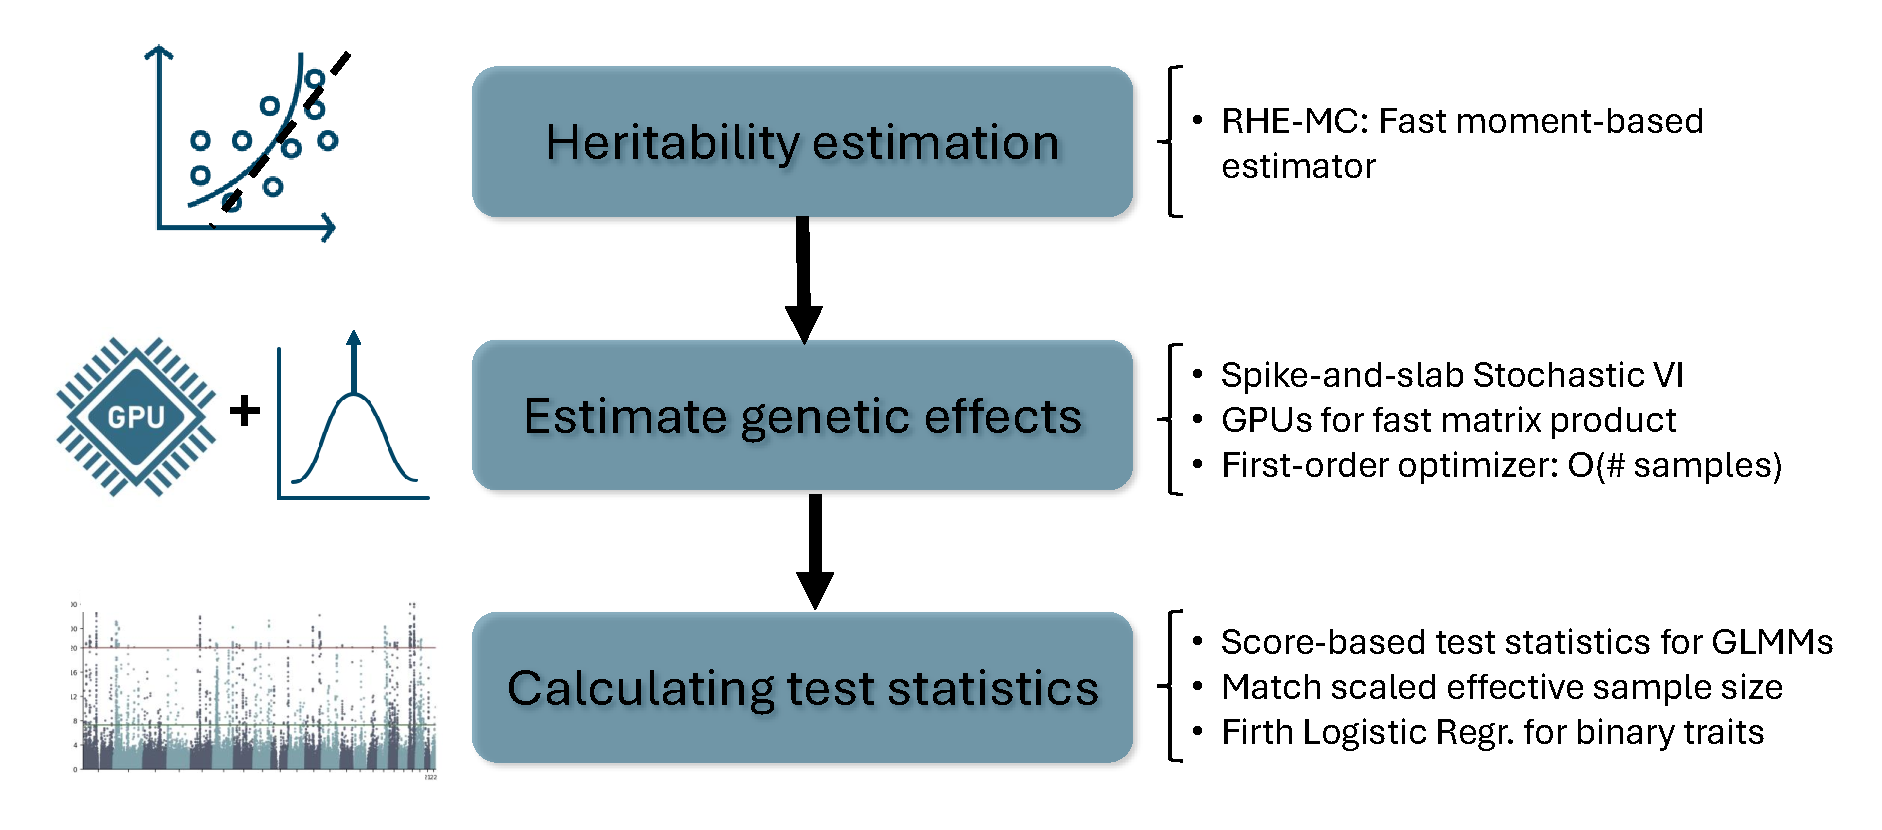
\includegraphics[width=\linewidth]{figures/thesis_qd_overview.pdf}
    \caption{\textbf{Overview of the Quickdraws algorithm.} The algorithm is divided into two main steps, first step deals with estimating genetic effects and the second step with calculating and calibrating per-variant test statistics. The first step is further divided into heritability estimation using moment-based methods \cite{zhu2024ARGRHE} and Bayesian regression for phenotype prediction which uses stochastic variational inference and GPU-based matrix multiplication for increased scalability. In the test statistics calculation step we use a novel calibration strategy which estimates and matches effective sample size with linear regression model run on unrelated and homogeneous subset of the data, along with approximate Firth logistic regression to correct for biases in binary traits. The illustrations were downloaded from Flaticon.}
    \label{fig:qd_overview}
\end{figure}

\subsection{Bayesian regression with spike-and-slab prior }
\label{sec:ch4-blr}
%
Quickdraws uses a Bayesian regression to estimate the genetic effects.
%
This Bayesian regression uses a spike-and-slab distribution on the variant effects, which results in increased association power compared to approaches that assume an infinitesimal model and rely on a Gaussian prior.
%
We optimize the posterior using stochastic variational inference \cite{hoffman2013stochastic}, which significantly improves the scalability of this approach.
%

\subsubsection{Quantitative traits}

Quickdraws adopts a Bayesian linear regression model as discussed in section \ref{sec:ch4-theory-mfvi}:
\begin{align}
    &\text{\textbf{Likelihood:} } &P(y \mid X, \beta) \sim \mathcal{N}(\beta^T X, \sigma_e^2) \nonumber \\
    &\text{\textbf{Prior:} } &P(\beta) = \prod_j P(\beta_j), \hspace{1mm} P(\beta_j) \sim (1-p_0)\mathcal{N} (0, \sigma ^ 2) + p_0 \delta(0) \nonumber \\
    &\text{\textbf{Approximate Posterior:} } &q(\beta) = \prod_j q(\beta_j), \hspace{1mm} q(\beta_j) \sim (1-\psi_j)\mathcal{N}(\mu_j, \sigma^2_j) + \psi_j \delta(0) \label{spike-and-slab-model2}
\end{align}

Similar to equation \ref{spike-and-slab-model}, given $N$ individuals and $M$ variants, $X$ is an $N \times M$ covariate-adjusted genotype matrix, $y$ is a $N \times 1$ covariate-adjusted phenotype vector, and $\beta$ is a $M \times 1$ vector of variant effects.
%
$\delta(0)$ is the Dirac delta function at 0, representing the spike in the spike-and-slab prior used to model the sparsity in the genetic architecture.
%
$\sigma_e^2$ and $\sigma^2$ are the variance component corresponding to environment and per predictor effect, $p_0$ is the sparsity and $j$ indexes over all model SNPs.
%
As we discussed in section \ref{sec:ch4-theory-mfvi}, we also assume a fully-factorized spike-and-slab approximate posterior, which leads to efficient and low-variance sampling from the posterior.
%
And, we use stochastic variational inference to directly optimize the evidence lower bound (ELBO).
%
The ELBO for Bayesian linear regression with spike-and-slab prior, normal likelihood, and spike-and-slab approximate posterior (derived in section \ref{sec:ch4-theory-svi}) can be approximated as follows: 
\begin{align}
    L^{Q}_{VI}&(\psi, \mu, \sigma) \approx - \sum\limits^{B}_{b=1} \Bigg( \sum\limits^{S}_{s=1} \frac{(y_b - \beta(s) X_b)^2}{2 \sigma_e^2} \ + \nonumber \\
    &+ \frac{1}{B}\sum\limits^{M}_{j=1} \left(  \frac{\psi_j}{2}\left(-1 + \frac{\mu_j^2 + \sigma_j^2}{\sigma^2} - \log \frac{\sigma_j^2}{\sigma^2} \right) + (1-\psi_j)\log\frac{1 - \psi_j}{1 - p_0} + \psi_j\log\frac{\psi_j}{p_0} \right) \Bigg) \label{elbo-loss-ss}
\end{align}

In this expression, $L^{Q}_{VI}(\psi, \mu, \sigma)$ is the variational inference objective to be maximized, $\psi, \mu, \sigma$ are the variational parameters to be optimized, $X_b$ and $y_b$ are a genotype matrix and a phenotype vector containing the $b^{th}$ (out of $B$) batch of the data, batched along the number of samples, while $\beta(s)$ are the effect estimates sampled from the approximate posterior $q(\beta)$.
%
Note that, contrary to other variational inference schemes, we aim to optimize a stochastic objective, since $\beta(s)$ is randomly sampled.
%

\subsubsection{Binary traits}
%
For binary traits, we adopt a Bayesian logistic regression model, so that the likelihood of Equation \ref{spike-and-slab-model2} becomes:
\begin{align}
    P(y \mid X, \beta) &= \prod_{n=1}^{N} c_n^{y_n} \{1 - c_n\}^{1-y_n}, \hspace{1mm} c_n = \sigma(\beta^T X_n),
    \label{spike-and-slab-model3}
\end{align}
while the prior and approximate posterior are unchanged.
%
In the above, $X_n$ and $y_n$ represent the covariate-adjusted genotype vector and phenotype values for the $n^{th}$ individual, $\sigma$ is the sigmoid function, which maps the output of the regression to a value between $0$ and $1$, and all other quantities are as previously defined.
%
We also assume that the approximate posterior has a spike-and-slab distribution; although it is not conjugate to the logistic distribution, we observed it to provide a good approximation to the true posterior.
%
The ELBO, which we again optimize using stochastic variational inference, now takes the form: 
\begin{align}
    L^{Bi}_{VI}&(\psi, \mu, \sigma) \approx - \sum\limits^{B}_{b=1} \Bigg( \sum\limits^{S}_{s=1} y_b \log(\sigma(\beta^T X_b)) + (1-y_b)\log(1-\sigma(\beta^T X_b)) \nonumber \ + \\
    &+ \frac{1}{B}\sum\limits^{M}_{j=1} \left(  \frac{\psi_j}{2}\left(-1 + \frac{\mu_j^2 + \sigma_j^2}{\sigma^2} - \log \frac{\sigma_j^2}{\sigma^2} \right) + (1-\psi_j)\log\frac{1 - \psi_j}{1 - p_0} + \psi_j\log\frac{\psi_j}{p_0} \right) \Bigg)
\end{align}

where all terms are defined as in Equation \ref{elbo-loss-ss} and derivation is provided in section \ref{sec:ch4-theory-svi}.

\subsubsection{Practical considerations}
Stochastic VI methods provide a principled and efficient way to perform variational inference.
%
This approach is simple but requires particular care to make sure that the variance of the ELBO estimate is not too large, as that may have a negative impact on convergence.
%
We make use of multiple recently developed strategies to reduce variance in the stochastic estimation of the ELBO, including continuous relaxation \cite{maddison2016concrete,jang2016categorical}, local reparameterization trick \cite{kingma2015variational}, and antithetic variates \cite{hammersley1956new}.

\vspace{2mm}

\noindent \textbf{Reparameterization:}
When dealing with stochastic objectives, such as the ELBO, it is often difficult to differentiate the objective due to intrinsic randomness in the parameters.
%
One solution to this problem is provided by the reparameterization trick \cite{kingma2013auto,blundell2015weight}, which models the stochasticity in the parameters as an input to the model rather than an intrinsic property of the model.
%
In more detail, the reparameterization trick assumes that distributions can be reparameterized in the form $g(\theta,\epsilon)$ where $\theta$ is the variational parameter, $\epsilon$ is the independently sampled random variable, and $g$ is a differentiable function.
%
As an example, consider the case of an isotropic normal distribution.
%
To sample from a mean-field normal distribution, we may reparameterize the sample as follows:
\begin{align}
    X &\sim \mathcal{N}(\mu, \sigma^2 I) \implies X = \mu + \epsilon \cdot \sigma, \nonumber \\
    \epsilon &\sim  \mathcal{N}(0, I),
\end{align}
where $\epsilon$ is i.i.d.\ normal noise with no dependence on $\mu$ and $\sigma$.
%
Relying on the reparameterization and treating $\epsilon$ as an independent input, we can differentiate with respect to $\mu$ and $\sigma$.
%

\vspace{2mm}
\noindent \textbf{Local reparamaterization:} The local reparamaterization trick \cite{kingma2015variational} was introduced as a way to provide computationally fast and low-variance gradient estimators in parameter-heavy stochastic VI methods.
%
It was originally applied to perform variational inference in Bayesian neural networks but is easily extended to Bayesian regression.
%
Using the original reparamaterization trick \cite{kingma2013auto,blundell2015weight} leads to sampling i.i.d.\ noise at least once for each parameter, making this approach computationally intensive in high-dimensional settings, which may involve millions of parameters.
%
The local reparamaterization trick translates the uncertainty on individual effect estimates, $\beta$, into local noise in the output, $\beta^T X$, thus reducing the computational overhead.
%
In the simple mean-field Gaussian VI, the local reparameterization trick can be used to sample the outputs directly,
\begin{align}
   &w_{i,j} \sim \mathcal{N}(\mu_{i,j}, \sigma^2_{i,j}), \hspace{4mm} b_{m,j} =  \sum_{i} a_{m,i} w_{i,j},
\end{align}
where $a_{m,i}$ is the $m$-th input data point and $b_{m,j}$ is the output corresponding to the $m$-th data point in the Bayesian linear regression model.
%
$b_{m,j}$ is a weighted-sum of normally distributed random variables, implying that $b_{m,j}$ is also normally distributed, with the following parameters:
\begin{align}
    &w_{i,j} \sim \mathcal{N}(\mu_{i,j}, \sigma^2_{i,j}) \implies b_{m,j} \sim \mathcal{N}(\gamma_{m,j}, \delta^2_{m,j}), \nonumber \\
    &\gamma_{m,j} = \sum_{i}a_{m,i}\mu_{i,j} ,\hspace{4mm}\delta^2_{m,j} =  \sum_{i}a^2_{m,i}\sigma^2_{i,j}.
\end{align}

In order to sample this output directly, one can apply the original reparameterization trick for the normal distribution:
\begin{align}
   b_{m,j} =  \gamma_{m,j} + \epsilon_{m,j} \delta_{m,j}, \hspace{4mm} \epsilon_{m,j} \sim \mathcal{N}(0, 1).
\label{eq:reparam_local}
\end{align}

Note that in Bayesian linear/logistic regression the local reparameterization removes the need to sample all the weights in a layer and only requires sampling proportional to the number of output variables for each mini-batch of data, substantially improving the computational complexity of the algorithm.
%
% Its important to note in Bayesian linear/logistic regression and Bayesian neural networks, the local reparameterization reduces sampling all the weights in the layer - $\mathcal{O}(N^2)$ to only sampling the pre-activations - $\mathcal{O}(N)$.

%
The local reparamaterization trick was originally only derived for mean-field Gaussian variational inference, since the weighted sum of arbitrary distributions cannot always be analytically derived.
%
In the case of mean-field spike-and-slab distributions, we use the central limit theorem to approximate the weighted sum of independent spike-and-slab distributions as approximately Gaussian.
%
Note that the input dimension for Bayesian regression in our setup is quite high (usually $>100,000$ markers), justifying this approximation.
%
% Thus, the central limit theorem provides a close approximation to the output of the model.
This idea was first explored in \cite{shayer2017learning} to sample discrete weights for binary and ternary neural networks.
% , relying on Lyapunov central limit theorems.
%
We thus reparametrize the output of our model (as described in equations \ref{spike-and-slab-model2} and \ref{spike-and-slab-model3}) as follows:
\begin{align}
    w_{i,j} &\sim p_{i,j}\mathcal{N}(\mu_{i,j}, \sigma^2_{i,j}) + (1 - p_{i,j})\delta(0) \implies b_{m,j} \sim \mathcal{N}(\gamma_{m,j}, \delta_{m,j}),  \nonumber \\
    \gamma_{m,j} &= \sum_{i}a_{m,i}\mu_{i,j}p_{i,j} ,\hspace{4mm}\delta_{m,j} =  \sum_{i}a^2_{m,i}(p_{i,j}\sigma^2_{i,j} + p_{i,j}\mu^2_{i,j} - p^2_{i,j}\mu^2_{i,j}).
\end{align}


\vspace{2mm}
\noindent \textbf{Antithetic variates for variance reduction:}
%
The use of antithetic variates is a popular approach to speed up Monte Carlo computations of the expectation of a random function \cite{hammersley1956new}.
%
This strategy relies on taking the antithetic path of the sampled path to reduce the variance in the overall estimator.
%
For example, in order to sample from a normal random variable (with mean $\mu$ and variance $\sigma^2$), one might use the reparameterization trick to sample $\mu +\epsilon \sigma$.
%
The antithetic path for a normally distributed random variable is $\mu - \epsilon \sigma$.
%
In addition to providing a valid sample from the underlying distribution (in this case, normal with mean $\mu$ and variance $\sigma^2$), the antithetic path also reduces the variance of the Monte Carlo estimate, as the sampled path and antithetic path are often negatively correlated.
%

%
We use both antithetic variates and the local reparameterization trick to reduce the variance of the ELBO.
%
As described above, the antithetic path for a normally distributed random variable is simply obtained by replacing $\epsilon$ with $-\epsilon$.
%
For each forward pass, we thus obtain two Monte Carlo samples for the output of the model as follows: 
\begin{align}
    \beta(s_1) &=  (\sum_{i}a_{m,i}\mu_{i,j} + \sqrt{\sum_{i}a^2_{m,i}(p_{i,j}\sigma^2_{i,j} + p_{i,j}\mu^2_{i,j} - p^2_{i,j}\mu^2_{i,j}} \epsilon ), \nonumber \\
    \beta(s_2) &= (\sum_{i}a_{m,i}\mu_{i,j} - \sqrt{\sum_{i}a^2_{m,i}(p_{i,j}\sigma^2_{i,j} + p_{i,j}\mu^2_{i,j} - p^2_{i,j}\mu^2_{i,j}} \epsilon ), \nonumber \\
    \beta(s) &= [\beta(s_1), \beta_2(s_2)].
\end{align}

\subsection{Heritability estimation}
\label{methods:h2}
%
To set the prior variance and likelihood contribution in equations \ref{spike-and-slab-model2} and \ref{spike-and-slab-model3}, we compute an estimate of the narrow-sense heritability for the trait of interest.
%
For quantitative traits, we estimate heritability using a parallelized implementation of the randomized Haseman–Elston regression algorithm\cite{wu2018scalable,pazokitoroudi2020efficient} (RHE, PyPI version 1.0) that allows the simultaneous estimation of variance components for multiple traits \cite{zhu2024ARGRHE}.
%
This approach requires a single pass through the data and allows estimating heritability in time linear in $N$ and $M$.
%
We set the number of random RHE-mc vectors to $50$ while assigning markers to $8$ components based on their LD scores and MAF. 
%
We also exclude the HLA region, as recommended in \cite{pazokitoroudi2020efficient}.
%
For Binary traits, we perform a grid search over a set of heritability values, $h2 \in \{0.01, 0.25, 0.5, 0.75\}$, running the Bayesian regression for each value and selecting the heritability corresponding to the highest likelihood.
%


\subsection{Test statistics calculation}
\label{methods:test_stats}
% talk about step1, now we do step 2
%
After estimating the random genetic effects as described in sections \ref{sec:ch4-blr} and \ref{methods:h2}, we compute association statistics for quantitative or binary traits as follows.
%
\subsubsection{Quantitative traits} 
%
We model the phenotype of interest as a combination of fixed and random effects, which include genetic effects and environmental effects:
\begin{equation}
    y = \alpha C + x_{test}\beta_{test} + g + \epsilon, \label{eq:lin_lmm}
\end{equation}
where $y$ is a $N \times 1$ vector of phenotype values, $x_{test}$ is a $N \times 1$ vector of variant values, $C$ is a $N \times C$ matrix of C covariates, $g$ and $\epsilon$ are random genetic and environmental effects.
%
Note that using a covariate-adjusted genotype and phenotype by first regressing out any covariates is equivalent to including covariates as fixed effects in the above equation.
%
Based on this model, we aim to compute the following $\chi^2$ association statistic (a derivation is provided in section \ref{sec:ch1-lmm}): 
\begin{equation}
   \frac{(x_{test}^T \hat{V}^{-1} y)^2}{x_{test}^T \hat{V}^{-1} x_{test}} \sim \chi^2_1, \label{lmm-chi2}
\end{equation}
where $\hat{V}$ is the estimated variance matrix, defined as $\hat{V} = \frac{\hat{\sigma_g}^2}{M} X_{GRM}X_{GRM}^T + \hat{\sigma_e}^2 I_N$, $\hat{\sigma_g}^2$ and $\hat{\sigma_e}^2$ are estimated genetic and environmental variance components, and $X_{GRM}$ is the genotype matrix used for model fitting.
%
Obtaining the test statistic of Equation \ref{lmm-chi2} requires calculating the inverse of a $N \times N$ matrix, which creates a computational bottleneck for large sample sizes.
%
This test statistic can be linked to the best linear unbiased predictor (BLUP) of a trait, by re-writing Equation \ref{lmm-chi2} as described in \cite{loh2015efficient}:
\begin{equation}
    \frac{(x_{test}^T \tilde{y}/\sigma_e^2)^2}{x_{test}^T \hat{V}^{-1} x_{test}} \sim \chi^2_1.
    \label{blup_lmm}
\end{equation}

%
In the above, $\tilde{y}$ is a residual phenotype estimated using BLUP.
%
We adopt a similar strategy and replace the $\tilde{y}$ with $\tilde{y}_{LOCO}$, leave-one-chromosome-out residual phenotype from Bayesian regression.
%
In addition, the denominator $x_{test}^T \hat{V}^{-1} x_{test}$ of Equation \ref{blup_lmm} can be shown to be well approximated using a constant multiple of $x_{test}^T x_{test}$ \cite{svishcheva2012rapid}, further reducing computational costs.
%
We can therefore write the test statistics for a quantitative trait up to a constant of proportionality as:
\begin{equation}
    \chi^2_{Q} \propto \frac{(x_{test}^T \tilde{y}_{LOCO})^2}{x_{test}^T x_{test}}.
    \label{chisq_test_2}
\end{equation}

\subsubsection{Binary traits}
%
For binary traits, we model the association between genotype and phenotype using a logistic mixed model:
\begin{equation}
    logit(p_i) = \alpha C + x_{test}\beta_{test} + g + \epsilon, \label{eq:log_lmm}
\end{equation}
where $p_i = P(y_i = 1 \mid x_{test}, g, C)$ is the probability of $i^{th}$ individual being a case given $x_{test}$, covariates $C$, and random genetic effects $g$.
%
A score test statistic for the null hypothesis $\beta_{test} = 0$ is then computed as $T = x_{test}^T(y - \hat{p})$, where $\hat{p}$ is the estimated mean under the null model.
%
The normalized test statistic for logistic mixed model can then be written as: 
\begin{equation}
    T = \frac{x_{test}^T(y - \hat{p})}{\sqrt{x_{test}^T\hat{P}x_{test}}},
\label{eq:log_lmm1}
\end{equation}
where $\hat{P} = \hat{V}^{-1} - \hat{V}^{-1} C(C^T\hat{V}^{-1}C)^{-1}C^T\hat{V}^{-1}$ is a dense $N \times N$ matrix with $\hat{V} = \frac{\hat{\sigma_g}^2}{M} X_{GRM}X_{GRM}^T + \hat{W}^{-1}$ and $\hat{W} = diag\{ \hat{p} (1-\hat{p}) \}$.
%
Similar to quantitative traits, the test statistic in Equation \ref{eq:log_lmm} can be written up to a constant of proportionality \cite{zhou2018efficiently} as:
\begin{equation}
    T_{B} \propto \frac{x_{test}^T(y - \hat{p})}{\sqrt{x_{test}^T\hat{W}x_{test}}},
\label{eq:log_lmm2}
\end{equation}
where $\hat{W}$ is a diagonal matrix (with diagonal entries $\hat{p_i} (1-\hat{p_i})$) from the predictions of the null model in Step 1.
%
The test statistic from \ref{eq:log_lmm2} is assumed to be normally distributed, which is often not the case with binary traits that have low prevalence or for rare variants.
%
We therefore instead perform Firth logistic regression, which penalizes the likelihood by using a Jeffreys' prior, removing most of the asymptotic bias in maximum-likelihood estimation.
%
In order to save computation, we use the likelihood ratio test with an approximate version of Firth logistic regression introduced in \cite{mbatchou2021computationally} on variants below a p-value threshold of 0.05. 
%
We further narrow down the list of variants by only applying Firth logistic regression to rare variants (default MAF $< 5\%$) or rare traits (default prevalence $< 5\%$) or both.

\subsubsection{Calibration of test statistics}

Calibrating the test statistics generated upto a constant of proportionality in equation \ref{chisq_test_2} and \ref{eq:log_lmm2} is a crucial part of a GWAS algorithm, which ensures the false positives are controlled.
%
We calibrate the summary statistics by estimating the effective sample size (ESS) increase compared to running linear regression on a homogeneous subset of unrelated individuals.
%
To this end, we estimate the increase in ESS linked to the use of non-infinitesimal Bayesian linear regression ($\gamma_{blr}$), as well as the reduction in ESS due to the presence of close relatives ($\gamma_{rel}$).
%
We then adjust the summary association statistics by matching the mean $\chi^2$ statistic minus one \cite{yang2011genomic} with that observed for linear or logistic regression run on a homogeneous subset of unrelated individuals.
%
In more detail, we multiply the uncalibrated Quickdraws summary statistics from equations \ref{chisq_test_2} and \ref{eq:log_lmm2} by a correction term $c$, computed as:
\begin{equation}
c = \frac{\gamma_{rel}\gamma_{blr}\frac{N_{qd}}{N_{lr}}(<\chi_{lr}^2> - 1) + 1}{<\chi_{qd}^2>}.
\label{eq:calib_main}
\end{equation}
In the above, $<\chi_{qd}^2>$ and $<\chi_{lr}^2>$ are the mean $\chi^2$ test statistics from Quickdraws and from linear/logistic regression run on a homogeneous unrelated subset of individuals, respectively.
%
$\frac{N_{qd}}{N_{lr}}$ is the ratio of the total number of samples to the number of homogeneous unrelated samples used for linear/logistic regression.
%
$\gamma_{rel}$ and $\gamma_{blr}$ are correction terms to account for relatedness and the use of Bayesian linear regression, which we describe in detail below.
%
Note that the $\gamma_{blr}$ term is estimated for each LOCO run, so the correction in equation \ref{eq:calib_main} is performed separately for each chromosome.
%
For binary traits, we use logistic regression and apply the correction separately for Firth-corrected and Firth-uncorrected variants.

\vspace{2mm}

%
\noindent \textbf{Correcting the ESS for the presence of relatedness ($\gamma_{rel}$ term).} To estimate the effective number of samples in the presence of relatedness, we follow an approach similar to that of \cite{ziyatdinov2021estimating}.
%
To this end, we first estimate genetic relatedness between samples using KING \cite{manichaikul2010robust} as implemented in PLINK \cite{chang2015second}.
%
We only retain relationships up to the 3rd degree (KING score $>2^{-\frac{9}{2}}$), as we found the ESS multiplier, described below, to not be significantly impacted by the inclusion of higher degree relatives.
%
For each pair of relatives, we estimate the degree of the relationship using KING’s output values as follows:

\begin{table}[h!]
\centering
\begin{tabular}{|c|c|}
\hline
\textbf{Range for KING $\psi$ value} & \textbf{Relatedness} \\
\hline
$\psi \geq 2^{-\frac{3}{2}}$ & 1 (Monozygotic Twins) \\
$2^{-\frac{3}{2}} > \psi \geq 2^{-\frac{5}{2}}$ & 0.5 ($1^{\text{st}}$ degree) \\
$2^{-\frac{5}{2}} > \psi \geq 2^{-\frac{7}{2}}$ & 0.25 ($2^{\text{nd}}$ degree) \\
$2^{-\frac{7}{2}} > \psi \geq 2^{-\frac{9}{2}}$ & 0.125 ($3^{\text{rd}}$ degree) \\
\hline
\end{tabular}
\caption{\textbf{Genetic relationship estimates based on KING values.}}
\label{tab:my_label}
\end{table}

Based on this, we compute the reduction factor for the effective sample size, $\gamma_{rel}$, using the following estimator, for which a derivation can be found in \cite{ziyatdinov2021estimating}:
\begin{equation}
\gamma_{rel} = \frac{tr((K \sigma_g^2 + I (1-\sigma_g^2))^{-1}K)}{N}.
\label{eq:calib_rel}
\end{equation}
In this expression, $N$ is the total number of samples, $K$ is the estimated kinship matrix, and $\sigma_g^2$ is the heritability of the trait.
%
To efficiently compute $\gamma_{rel}$, we eigendecompose the matrix $K$, obtained using KING utilizing the block-like structure of the kinship matrix. 
%
In particular, the effective sample size multiplier in the presence of relatedness can be approximated as:
\begin{equation}
\gamma_{\text{rel}} \approx \frac{1}{N}\sum\limits_{i=1}^{N} \frac{\lambda_i}{(\lambda_i - 1)\sigma_g^2 + 1},
\end{equation}
where $\lambda_i$ is the $i^{\text{th}}$ eigenvalue of the kinship matrix $K$.
%
And to facilitate this computation, we separately sum across each block $B_i$ of related individuals:
\begin{equation}
\gamma_{\text{rel}} \approx \frac{1}{N} \sum\limits_{i=1}^{B} \sum\limits_{j=1}^{N_{B_i}} \frac{\lambda_{i,j}}{(\lambda_{i,j} - 1)\sigma_g^2 + 1}.
\end{equation}
%
For binary traits, we convert the heritability from the liability scale to the observed scale.
%

\vspace{2mm}

%
\noindent \textbf{Correcting the ESS for the use of Bayesian linear regression ($\gamma_{blr}$ term):}
%
The effective sample size multiplier, $\gamma_{blr}$, has been shown to be proportional to the inverse of the residual trait variance in a linear regression model \cite{loh2015efficient, ziyatdinov2021estimating}.
%
To account for the increase in effective sample size in the model fitting step, we therefore calculate the inverse variance of the residual trait 
\begin{equation}
    \gamma_{blr} = \frac{Var(y)}{Var(y-\hat{y})}
\end{equation}
where $y$ and $\hat{y}$ are true and predicted trait values from the whole-genome regression regression on a held-out set.
%
In more detail, we use the effect estimates from the best sparsity parameter to calculate the variance explained on held-out data.
%
As the $\gamma_{blr}$ term needs to be computed during the LOCO step, we compute these variance terms separately for each chromosome and sum across all chromosomes, excluding the one currently being tested.
%


\subsection{Performance optimization}
\subsubsection{Memory optimization}
\begin{enumerate}
    \item \textbf{Raw genotypes:}
    %
    for a diploid individual, the raw genotypes take values in ${0,1,2}$.
    %
    We store the $N \times M$ genotype matrix in $NM/4$ bytes, i.e. using 2 bits per genotype entry.
    %
    We do so by encoding 8 consecutive entries of the genotype matrix using two 8-bit integers using the built-in \texttt{numpy} features in Python, \texttt{np.packbits()} and \texttt{np.unpackbits()}.
    %
    We also store the column-wise mean and variance of the genotype matrix, used to mean-center and standardize, on the fly.
    %
    
    \item \textbf{Genotype streaming during the calculation of test statistics:}
    %
    the calculation of test statistics is usually performed on many more variants than those used for model fitting.
    %
    We therefore optimize this step by streaming genotype blocks rather than loading all the variants into memory.
    %
    The block size is determined based on the maximum memory allowed at runtime (default: 32GB) and the data IO is parallelized using multiple cores.
    %
    
\end{enumerate}

%% Handle raw genotypes, saved in HDF5 file for speedy access
%% Streaming genotype rathern than loading it
\subsubsection{Speed optimization}
\begin{enumerate}
    \item \textbf{GPUs for fast Bayesian regression:} we use GPUs along with the \texttt{pytorch} machine learning package \cite{paszke2017automatic} to speed-up matrix multiplication and sampling operations during stochastic variational inference.
    %
    % We observed by using GPUs we were able to speed-up the matrix multiplication and sampling bottlenecks thereby making our Bayesian regression much faster than just using CPUs. 
    % We benchmark the speed gain in whole-genome regression and compare on two popular GPU models: Nvidia A100 and Nvidia 3080.  
    % Add figure comparing performance gain due to using GPUs vs CPUs
    \item \textbf{Transfer learning:} rather than training the $22$ LOCO models independently, we initialize each model training using the effect estimates previously computed for the whole-genome regression.
    %
    This transfer learning approach requires fewer iterations to converge, making model fitting $2\times$ to $2.5\times$ faster, and leads to similar association power when compared to training each LOCO model separately.
    %
    We compare the advantage of transfer learning over independent random initialization in simulations, by looking at the power improvement vs number of iterations in Figure \ref{fig:transfer}.

    \begin{figure}[h]
    \centering
    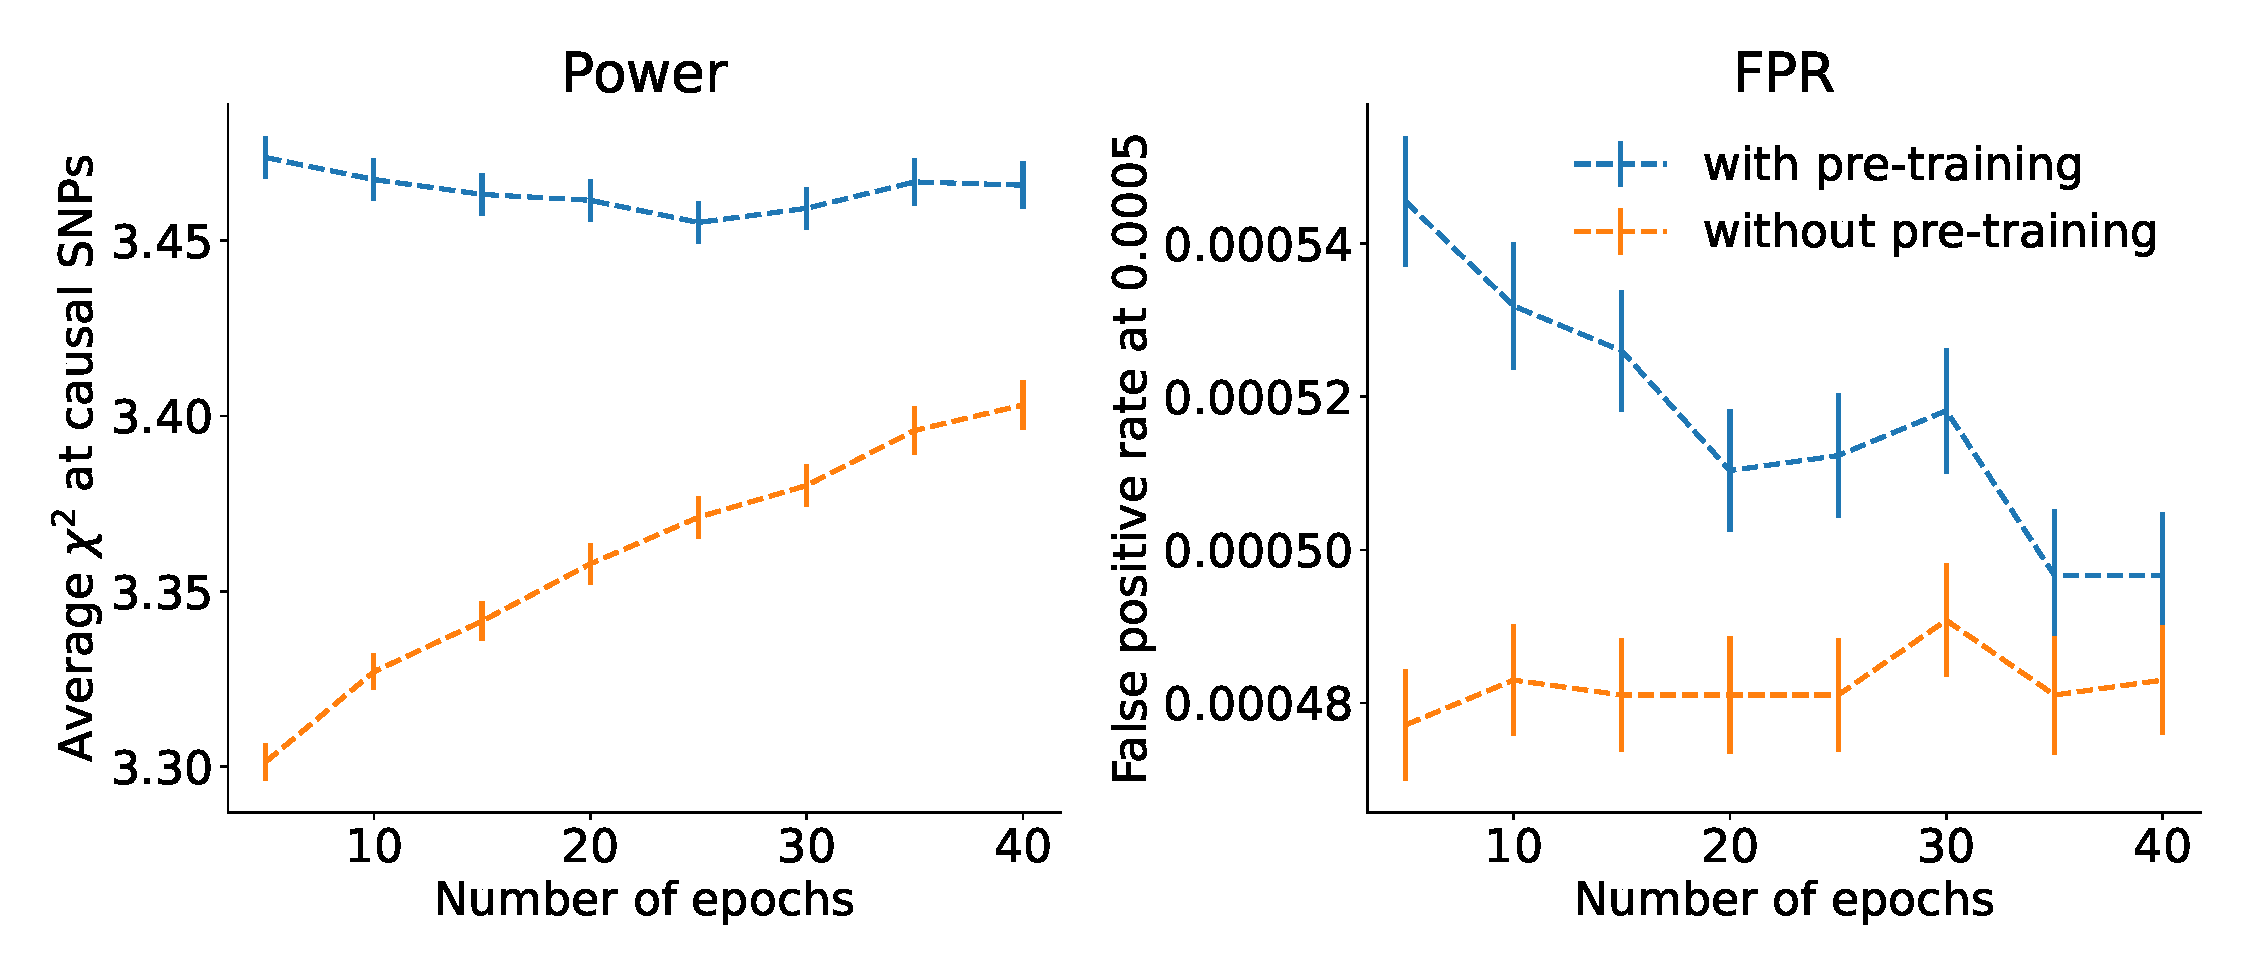
\includegraphics[width=\textwidth]{figures/transfer.pdf}
    \caption{\textbf{
    %
    Transfer-learning in Bayesian regression.}
    %
    We measure the causal $\chi^2$ and false positive rate at $5 \times 10^{-4}$, with and without pre-training (for $90$ epochs), and varying the number of LOCO training epochs.
    %
    Error bars represent the standard error of the mean $\chi^2$ or false positive rate across $50$ independent quantitative traits with GB-unrel structure and $2\%$ polygenicity.
    %
    }
    \label{fig:transfer}
\end{figure}
    

    \item \textbf{Numba optimization for the calculation of test statistics:}
    %
    we implement a fully-vectorized version of linear regression for multiple traits using the \texttt{parallel} and \texttt{njit} functionality from the Numba just-in-time (JIT) compiler \cite{lam2015numba}.
    %
    % Numba is able to escape the global interpreter lock in python, making the code able to compile without involving any interpreter - this along with prebuilt numpy features makes the python code as fast as a C or C++ implementation of it. 
    \item \textbf{Calibrating test statistics using genotyped SNP data:}
    %
    instead of running linear regression or logistic regression on all imputed variants, we calibrate our test statistics only using the genotype data provided in step 1 (${\sim}458k$ variants).
    %
    We find that matching scaled effective sample size estimates using this subset of variants provides consistent calibration in the larger set of imputed variants, while greatly reducing running time, as we only need to evaluate the logistic or linear regression model on a subset of variants.
    %
    \item \textbf{HDF5 and PySnpTools for data loading:}
    %
    we store the raw genotype matrix in a compressed HDF5 file \cite{hdf5}, which provides fast sample-wise access (i.e., it allows obtaining all variants for an individual) for Bayesian regression.
    %
    We instead use PySnpTools (see \url{https://github.com/fastlmm/PySnpTools}), which provides parallelizable variant-wise access, to access \texttt{bgen} or \texttt{bed} files for the calculation of test statistics. 
    \item \textbf{Approximate Firth logistic regression:} Approximate Firth regression is only applied to variants with logistic regression p-value below $0.05$, as done in Regenie and FastGWA-GLMM.
    %
    We further narrow down the list of variants by only applying Firth logistic regression to rare variants (MAF < 5\%) or rare traits (prevalence < 5\%).
    %
    \item \textbf{Multiple traits:} Most of our operations are vectorized using Numpy \cite{harris2020array} and Numba \cite{lam2015numba}, which leads to computational gains in the parallel analysis of multiple traits.
    %
\end{enumerate}

\subsection{Hyperparameter tuning}
We perform cross-validation by randomly splitting the data into training ($80\%$) and testing ($20\%$) sets to estimate the optimal sparsity hyperparameter $1-p_0$ (see Equation \ref{spike-and-slab-model}) using the values $\{0.5, 0.2, 0.1, 0.05, 0.02, 0.01\}$.
%
For heritability in binary traits, we evaluate $\{0.01, 0.25, 0.5, 0.75 \}$.
%
Compared to coordinate-ascent variational inference, stochastic variational inference relies on additional hyperparameters that affect the final testing performance.
%
These include the learning rate of the optimizer, the batch-size, and the number of training epochs.
%
Setting a high learning rate results in unstable convergence of the optimizer, while a low learning rate leads to the need for more training epochs.
%
Larger batch sizes lead to better performance but increased GPU memory usage.
%
Considering these trade-offs, we set the batch-size to $128$; the learning rate corresponding to each value of the sparsity hyperparameter was set to $4 \times 10^{-4}$, $2 \times 10^{-4}$, $2 \times 10^{-4}$, $1 \times 10^{-4}$,$2 \times 10^{-5}$, $5 \times 10^{-6}$ for sparsity ($1-p_0$) $ \in \{0.01, 0.02, 0.05, 0.1, 0.2, 0.5\}$.
%
We also set the number of training epochs to $80$ for the initial cross-validation step, and to $40$ for the final LOCO step.
%
We observed these hyperparameters to be robust across various sample sizes, providing a good balance between statistical power and computational costs. 

\newpage

\section{Summary of the Quickdraws algorithm}
\label{sec:ch4-summary}
%
We provide a summary of the Quickdraws algorithm, which performs two main steps:
%
\begin{enumerate}
    \item \textbf{Estimating genetic effects (model fitting):} This is further divided into two parts:
    \begin{enumerate}
        \item \textbf{Variance component estimation:}
        %
        For quantitative traits, we use a multi-trait version of the RHE-mc algorithm \cite{wu2018scalable,pazokitoroudi2020efficient,zhu2024ARGRHE} to obtain estimates of narrow-sense heritability.
        %
        For binary traits, we directly perform the Bayesian regression (see below) while testing several heritability values in a grid search.
        %
        \item \textbf{Bayesian regression: }
        %
        We perform Bayesian linear/logistic regression to estimate the genetic effects, using a spike-and-slab prior on the effect estimates:
        \begin{equation}
            P(\beta_j) \sim (1-p_0)\mathcal{N} (0, \sigma ^ 2) + p_0 \delta(0).
        \end{equation}
        
        %
        There is one free hyperparameter in the prior (the sparsity term $1-p_0$) for quantitative traits and two free hyperparameters for binary traits (the sparsity term and $h^2$).
        %
        We perform cross-validation to estimate these hyperparameters, splitting the input genotype/phenotype data into $90\%$ for training and $10\%$ for validation and parallelly running the regression using $1-p_0 \in \{0.01, 0.02, 0.05, 0.1, 0.2, 0.5\}$ and, for binary traits, $h^2 \in \{0.01, 0.25, 0.5, 0.75, 0.9 \}$.
        %
        We choose the sparsity (and $h^2$ for binary traits) parameter that maximizes (in the validation set) the test log-likelihood for the traits.
        %

        %
        After obtaining the optimal hyperparameters for each trait, we retrain the regression using a leave-one-chromosome-out approach.
        %
        We obtain a $2.5-3 \times$ speed-up for the training for this LOCO step by using transfer learning, initializing the effect estimates from the cross-validation run performed using all chromosomes.
        %
    \end{enumerate}
    %    
    \item \textbf{Calculation and calibration of association statistics (testing):}
    %
    Given the estimated genetic effects, we calculate linear mixed-model or logistic mixed-model test statistics up to a constant of proportionality.
    %
    We rely on optimizations such as just-in-time compilation and code vectorization in Numba.
    %
    We estimate the constant of proportionality by matching the estimated scaled effective sample size of linear regression on a subset of unrelated homogeneous samples for quantitative traits, and logistic regression on a subset of unrelated homogeneous samples for binary traits.
    %
\end{enumerate}